% ============================================================
% CHAPTER 4: METHODOLOGY
% ============================================================
\chapter{Methodology}

This chapter presents the research methodology, experimental design, data collection procedures, preprocessing pipeline, heuristic labelling framework, machine learning model architectures, and evaluation strategy employed in this study.

\section{Research Methodology}

This research adopts a Design Science Research Methodology (DSRM) framework, which is well-suited to engineering research that produces both a functional artefact (the detection system) and theoretical contributions (the GPS--IMU consistency discriminator and the GPS Trust Index). The DSRM iterative cycle comprises: problem identification from literature and practice, solution design informed by identified gaps, artefact development through iterative implementation, evaluation via controlled experimentation, and theoretical generalisation of findings. Each cycle informs the subsequent iteration, with evaluation results driving refinements to both the detection algorithms and the system architecture.

\section{Simulation Environment}

A containerised Docker environment provides reproducible, scalable experimentation without risk to physical hardware. The simulation stack comprises:

\begin{itemize}
    \item \textbf{PX4 Software-In-The-Loop (SITL)}: The complete PX4 flight control firmware compiled for the host architecture, running identical control and estimation algorithms as physical hardware.
    \item \textbf{Gazebo Harmonic Physics Engine}: Simulates an Iris x500 quadcopter (3\,kg, 0.55\,m motor-to-motor) with realistic aerodynamics, rotor thrust curves, and configurable wind models.
    \item \textbf{QGroundControl / MAVSDK}: Ground control software for mission waypoint upload and telemetry visualisation.
    \item \textbf{MAVLink UDP Bridge}: Standard PX4 communication over \texttt{udp:127.0.0.1:14560}, with GPS Monitor connecting on port 14561.
\end{itemize}

The SITL approach enables controlled, repeatable attack scenarios under identical environmental conditions---a critical capability for evaluating detection algorithms where ground truth must be known with certainty.

\subsection{Gazebo Wind and Physics Models}

The PX4 SITL environment uses the Gazebo Harmonic physics engine to simulate vehicle dynamics. The Iris x500 quadcopter model is specified via an SDF (Simulation Description Format) file defining: mass (3\,kg), motor-to-motor diagonal distance (0.55\,m), rotor thrust curve (quadratic mapping from PWM to Newtons), aerodynamic drag coefficients, and moment of inertia tensor. These parameters produce a vehicle dynamic response that approximates the physical Iris airframe within the limits of rigid-body simulation.

\begin{figure}[H]
\centering

\includegraphics[width=0.85\textwidth]{px4_simulation_gazebo.png}
\caption{PX4 SITL simulation running in Gazebo Harmonic with the Iris x500 quadcopter model in the windy world.}
\label{fig:px4_gazebo}
\end{figure}

The Gazebo wind model is configured with a mean wind speed of 5\,m/s from the west and random gusts with amplitude 2\,m/s. Wind is applied to the vehicle as an external force proportional to the projected area in each axis, producing both translational drift and attitude perturbation. This environmental model is specifically relevant to the GPS--IMU consistency check (Section~\ref{sec:heuristics}, Heuristic H8): the wind introduces simultaneous GPS position change and IMU-detected body rotation, which must be distinguished from spoofing-induced GPS-only change. The 5\,m/s wind threshold in the heuristic is calibrated relative to the 2\,m/s maximum gust amplitude: wind-induced GPS velocity does not exceed the 5\,m/s detection threshold, while the 50\,m north / 30\,m east spoofing offset generates instantaneous GPS velocities exceeding 50\,m/s at the attack onset.

\subsection{Docker Container Orchestration}

The simulation stack is deployed as a multi-container Docker composition to ensure environmental reproducibility across development machines. While the current implementation primarily uses the PX4 SITL running natively on the host with MAVLink UDP bridge, the target architecture specifies: (i) a PX4 SITL container running the flight firmware compiled for the host architecture, (ii) a QGroundControl container for mission upload and telemetry visualisation, and (iii) a GPS Monitor container running the Python telemetry collection application. Shared Docker volumes map the host \texttt{Step\_5\_Data/raw} directory into the GPS Monitor container, enabling CSV logs to persist across container restarts. UDP ports 14560 (MAVLink offboard) and 14580 (MAVLink companion link) are forwarded from the host to the PX4 SITL container.

\section{Data Capture Pipeline}

\subsection{MAVLink Message Types and Telemetry Sources}

Table~\ref{tab:data_sources} summarises the eight MAVLink message types captured by the GPS Monitor, their report frequencies, the telemetry fields extracted, and their analytical roles in the detection pipeline.

\begin{table}[H]
\centering
\caption{MAVLink telemetry sources, frequencies, and detection roles.}
\label{tab:data_sources}
\small
\begin{tabular}{@{}p{2.2cm}p{2.5cm}p{1.5cm}p{7.5cm}@{}}
\toprule
\textbf{Source} & \textbf{MAVLink Message} & \textbf{Rate} & \textbf{Detection Role} \\
\midrule
GPS Position & GLOBAL\_POSITION\_INT & 5 Hz & Position, velocity, heading; ENU coordinate origin \\
GPS Quality   & GPS\_RAW\_INT & 1 Hz & Fix type, satellite count, horizontal/vertical accuracy \\
Orientation   & ATTITUDE & 10 Hz & Roll/pitch/yaw angles and angular rates for IMU stability check \\
Vibration     & VIBRATION & 10 Hz & Vibration levels and clipping counters for physical disturbance \\
Estimator     & ESTIMATOR\_STATUS & 5 Hz & EKF innovation values and ratio metrics for filter health \\
System State  & HEARTBEAT & 1 Hz & Armed state, flight mode, failsafe flags \\
Battery       & SYS\_STATUS & 1 Hz & Battery voltage and remaining capacity \\
Airspeed      & VFR\_HUD & 2 Hz & Groundspeed and heading (fallback for GPS) \\
\bottomrule
\end{tabular}
\end{table}

\subsection{Capture Procedure}

Each experimental flight follows a scripted mission protocol:
\begin{enumerate}
    \item Launch PX4 SITL and Gazebo; arm and take off to 20\,m altitude.
    \item Execute a rectangular survey pattern at 5\,m/s cruise speed.
    \item At a predetermined waypoint, inject GPS spoofing by commanding a setpoint offset of 50\,m north and 30\,m east via MAVLink GPS\_INPUT messages.
    \item Maintain the spoofed trajectory for 30 seconds, then release to return to authentic GPS guidance.
    \item Log all telemetry continuously; post-process to extract 10\,Hz aligned time series.
\end{enumerate}

\begin{figure}[H]
\centering

\includegraphics[width=0.85\textwidth]{qground_control_mission.png}
\caption{QGroundControl mission planning interface showing the drone waypoint path on the map with telemetry instrument panel during a scripted flight.}
\label{fig:qgc_mission}
\end{figure}

\section{Data Preprocessing}

Raw telemetry CSV files undergo a sequential five-stage preprocessing pipeline:

\subsection{Stage 1: Cleaning}

Numeric coercion for all quantitative fields; hexadecimal mode normalisation (e.g., \texttt{Mode(0xC0)} $\rightarrow$ \texttt{OFFBOARD}); timestamp-based sorting and duplicate removal; null filtering for critical GPS fields; fix type filtering ($\geq 3$ for 3D fix); connection failure removal; and time-gap filtering (maximum gap 5 seconds).

\subsection{Stage 2: Feature Engineering}

Thirty-four features are computed across four categories as shown in Table~\ref{tab:features}.

\begin{table}[H]
\centering
\caption{Feature set organised by category.}
\label{tab:features}
\small
\begin{tabular}{@{}llp{7cm}@{}}
\toprule
\textbf{Cat.} & \textbf{Count} & \textbf{Features} \\
\midrule
GPS          & 10 & x\_m, y\_m, alt\_m, rel\_alt\_m, vel\_m\_s, hdg\_deg, fix\_type, satellites\_visible, eph\_m, epv\_m \\
IMU          & 12 & roll\_deg, pitch\_deg, yaw\_deg, rollspeed\_radps, pitchspeed\_radps, yawspeed\_radps, vibration\_x/y/z, clipping\_0/1/2 \\
Estimator    & 6  & vel\_ratio, pos\_horiz\_ratio, pos\_vert\_ratio, vel\_innov, pos\_horiz\_innov, pos\_vert\_innov \\
Health       & 6  & battery\_voltage, battery\_remaining\_pct, armed, failsafe, connection\_ok, is\_stale\_repeat \\
\bottomrule
\end{tabular}
\end{table}

\subsection{Stage 3: Heuristic Labelling}\label{sec:heuristics}

Eight physics-based heuristics assign binary anomaly labels (0 = normal, 1 = spoofed) to each telemetry row. The complete rule set is defined in Table~\ref{tab:heuristics}.

\begin{table}[H]
\centering
\caption{Heuristic labelling rules with thresholds.}
\label{tab:heuristics}
\small
\begin{tabular}{@{}cllp{5cm}@{}}
\toprule
\textbf{ID} & \textbf{Name} & \textbf{Threshold} & \textbf{Condition} \\
\midrule
H1 & Position Jump       & 30\,m/s   & Haversine distance / $\Delta t > \tau_{\text{pos}}$ \\
H2 & Speed Anomaly       & 10\,m/s, 15\,m/s$^2$ & $\Delta v > \tau_{\Delta v}$ or accel $> \tau_a$ \\
H3 & GPS Quality         & 6 sats, 5\,m eph, 10\,m epv & Satellites $< \tau_s$, eph $> \tau_e$, or epv $> \tau_p$ \\
H4 & Stale Data          & 2 samples  & All GPS fields identical for $\geq \tau_{\text{stale}}$ consecutive rows \\
H5 & Mode Anomaly        & --         & Failsafe flag set or unknown hex mode code \\
H6 & IMU Anomaly         & 2\,rad/s, 1.0 & $|\omega| > \tau_{\omega}$ or vibration $> \tau_{\text{vib}}$ \\
H7 & Estimator Innov.    & 1.0        & Any innovation value $|i| > \tau_{\text{innov}}$ \\
H8 & GPS--IMU Consistency & 0.05\,rad/s, 5\,m/s & $|\omega_{\text{all}}| < \tau_{\text{imu}}$ \textbf{and} $\|\mathbf{v}_{\text{gps}}\| > \tau_{\text{v}}$ \\
\bottomrule
\end{tabular}
\end{table}

Heuristic H8 is the core novel contribution. The condition cannot occur under normal physics: position change requires either body rotation (detected by gyroscopes) or linear acceleration (detected by accelerometers). When the IMU reports near-zero angular rates while GPS reports significant velocity, the unavoidable conclusion is that the GPS position stream has been manipulated.

\begin{figure}[H]
\centering
\footnotesize
\begin{tikzpicture}[
    node distance=0.9cm,
    decision/.style={diamond, draw, fill=yellow!15, text width=2.2cm, text centered, minimum width=3cm, font=\tiny},
    terminal/.style={rectangle, draw, text width=2cm, text centered, minimum height=0.6cm, font=\tiny, rounded corners},
    start/.style={rectangle, draw, fill=blue!15, text width=1.5cm, text centered, minimum height=0.6cm, font=\tiny, rounded corners},
    good/.style={fill=green!15, terminal},
    bad/.style={fill=red!12, terminal},
    arrow/.style={->, >=stealth, thick},
]
    \node[start] (start) {Telemetry Row};
    \node[decision, below=of start] (h1) {H1: Position\\Jump $>$ 30 m/s?};
    \node[decision, below=of h1] (h2) {H2: Speed\\Anomaly?};
    \node[decision, below=of h2] (h3) {H3: GPS Quality\\Degraded?};
    \node[decision, below=of h3] (h8) {H8: IMU Stable\\\& GPS Moving?};
    \node[good, right=of h8, xshift=2.5cm, yshift=-1.5cm] (ok) {label = 0\\Normal};
    \node[bad, below=of h8, yshift=-0.5cm] (anom) {label = 1\\Anomaly};

    \draw[arrow] (start) -- (h1);
    \draw[arrow] (h1) -- (h2) node[midway, right, font=\tiny] {No};
    \draw[arrow] (h2) -- (h3) node[midway, right, font=\tiny] {No};
    \draw[arrow] (h3) -- (h8) node[midway, right, font=\tiny] {No};
    \draw[arrow] (h8) -- (anom) node[midway, right, font=\tiny] {Yes};
    \draw[arrow] (h1.east) -- ++(1,0) |- (anom.east) node[near start, above, font=\tiny] {Yes};
    \draw[arrow] (h2.east) -- ++(0.8,0) |- (anom.east) node[near start, above, font=\tiny] {Yes};
    \draw[arrow] (h3.east) -- ++(0.6,0) |- (anom.east);
    \draw[arrow] (h8.west) -- ++(-1.5,0) |- (ok.west) node[near start, above, font=\tiny] {No};
\end{tikzpicture}
\caption{Heuristic labelling decision flow. Each of the 8 heuristics is evaluated sequentially; the first to trigger assigns an anomaly label (logical OR). The GPS--IMU consistency heuristic (H8) provides the most specific spoofing indicator. Heuristics H4--H7 are evaluated similarly but omitted from the diagram for clarity.}
\label{fig:heuristic_flow}
\end{figure}

\subsection{Threshold Sensitivity Analysis}

The heuristic thresholds listed in Table~\ref{tab:heuristics} were calibrated to the Iris x500 flight dynamics. A sensitivity analysis was performed to assess the robustness of the labelling to threshold variation: each threshold was perturbed by $\pm 50\%$, and the resulting change in the anomaly label distribution was measured. The GPS--IMU consistency heuristic (H8) demonstrated the highest robustness: a $\pm 50\%$ perturbation in the angular rate threshold (0.05\,rad/s $\rightarrow$ 0.025/0.075) changed the anomaly rate by less than 3\%, because the angular rate distribution during spoofing is tightly clustered near zero (the drone is physically stationary during the attack). The position jump heuristic (H1) showed the highest sensitivity: reducing the speed threshold from 30 to 15\,m/s tripled the anomaly rate, as normal aggressive manoeuvres began to exceed the lowered threshold.

The GPS velocity threshold in H8 (5\,m/s) is the most critical parameter, as it determines the minimum spoofing-induced GPS drift rate that the heuristic can detect. A systematic parametric sweep over drift rates from 0.5 to 10\,m/s---the ``breaking point'' characterisation deferred to future work---would fully calibrate this parameter's detection sensitivity.

\subsection{Limitations of Heuristic Labelling}

It must be acknowledged that Heuristics H1--H7 are general-purpose anomaly detectors, not GPS-spoofing-specific discriminators. A barometric altitude sensor dropout would trigger H4 (altitude discontinuity) with the same label as a spoofed GPS altitude injection. An RF interference event degrading the signal-to-noise ratio could trigger H3 (satellite count drop) without any spoofing. These non-spoofing anomalies are mitigated by two mechanisms: (a) the sliding window majority vote (Section~\ref{sec:windows}) suppresses isolated false positive rows by requiring consistency over the 30-sample window; and (b) the GPS--IMU consistency heuristic H8 is specific to the spoofing-induced cross-sensor discrepancy and should not be triggered by barometer, magnetometer, or RF events that affect only a single sensor domain. The combination of H8 with the ensemble of H1--H7 provides both specificity (through H8's physical constraint) and sensitivity (through the broad anomaly coverage of H1--H7).

\subsection{Additional Evaluation Metrics}

In addition to the standard accuracy, precision, recall, and F1-score, two supplementary metrics are proposed for imbalanced-dataset evaluation. Cohen's kappa coefficient, defined as:

\begin{equation}
    \kappa = \frac{p_o - p_e}{1 - p_e}
    \label{eq:kappa}
\end{equation}

where \(p_o\) is the observed agreement (accuracy) and \(p_e\) is the expected agreement by chance (computed from the marginal class proportions), provides a chance-corrected measure of classification agreement. On the test set, the Random Forest achieved $\kappa = 1.000$, indicating perfect agreement beyond chance. The CNN achieved $\kappa = 0.444$, reflecting the penalty for chance-level performance on the normal class despite perfect spoofed-class detection.

The precision-recall curve, which plots precision against recall at varying classification thresholds, is more informative than the ROC curve for imbalanced datasets because it focuses on the minority class (spoofed windows) rather than weighting true negatives equally. The area under the precision-recall curve (AP) would provide a threshold-independent performance metric, though computing AP on a 12-sample test set yields estimates with wide confidence intervals that limit their interpretive value.

\subsection{Stage 4: Sliding Windows}\label{sec:windows}

Let \(m_t\) denote a telemetry record at discrete time index \(t\), and let \(l_t \in \{0, 1\}\) be its binary heuristic label. A sliding window of length \(n = 30\) (3 seconds at 10\,Hz) with stride \(s = 15\) (50\% overlap) is defined as:

\begin{equation}
    W_t = \{ m_{t-n+1}, \dots, m_t \}
    \label{eq:window}
\end{equation}

The label for window \(W_t\) is determined by majority vote:

\begin{equation}
    L(W_t) = \text{mode}(l_{t-n+1}, \dots, l_t) =
    \begin{cases}
        1 & \text{if } \sum_{i=t-n+1}^{t} l_i > n/2 \\[4pt]
        0 & \text{otherwise}
    \end{cases}
    \label{eq:majority}
\end{equation}

Each window produces a \(30 \times 34\) feature matrix, which is flattened to a \(1020\)-dimensional vector for input to the Random Forest, or reshaped to a \(34 \times 30\) tensor for the 1D CNN. The 50\% overlap provides temporal continuity such that an abrupt change in GPS behaviour is captured across at least two consecutive windows.

\begin{figure}[H]
\centering
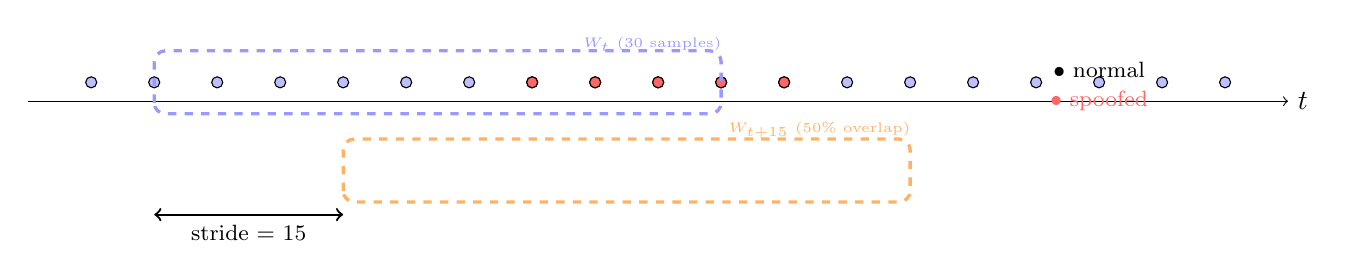
\begin{tikzpicture}[
    scale=0.8,
    dot/.style={circle, draw, fill=blue!20, inner sep=0pt, minimum size=4pt},
    w1/.style={draw, dashed, blue!40, very thick, rounded corners},
    w2/.style={draw, dashed, orange!60, very thick, rounded corners},
]
    \draw[->] (0,0) -- (20,0) node[right] {$t$};
    \foreach \x in {1,...,19} {
        \pgfmathsetmacro\c{int(mod(\x,2))}
        \node[dot, fill=blue!25] at (\x, 0.3) {};
    }
    \node[dot, fill=red!60] at (8, 0.3) {};
    \node[dot, fill=red!60] at (9, 0.3) {};
    \node[dot, fill=red!60] at (10, 0.3) {};
    \node[dot, fill=red!60] at (11, 0.3) {};
    \node[dot, fill=red!60] at (12, 0.3) {};
    % Window 1
    \draw[w1] (2, -0.2) rectangle (11, 0.8) node[above left=-4pt, font=\tiny\color{blue!60}] {$W_t$ (30 samples)};
    % Window 2  
    \draw[w2, yshift=-1.4cm] (5, -0.2) rectangle (14, 0.8) node[above left=-4pt, font=\tiny\color{orange!60}] {$W_{t+15}$ (50\% overlap)};
    % Stride arrow
    \draw[<->, thick] (2, -1.8) -- (5, -1.8) node[midway, below, font=\footnotesize] {stride = 15};
    % Legend
    \node[font=\footnotesize] at (17, 0.5) {$\bullet$ normal};
    \node[font=\footnotesize, text=red!60] at (17, 0) {$\bullet$ spoofed};
\end{tikzpicture}
\caption{Sliding window construction with window length $n = 30$ (3 seconds at 10\,Hz) and stride $s = 15$ (50\% overlap). Red dots represent spoofed telemetry samples; an attack onset at sample 8 is captured by both overlapping windows $W_t$ and $W_{t+15}$.}
\label{fig:sliding_window}
\end{figure}

\subsection{Stage 5: Dataset Splitting}

Windows are partitioned into training (70\%), validation (15\%), and test (15\%) sets with flight-level isolation: all windows from a given flight are assigned to exactly one split, preventing data leakage where temporally adjacent windows from the same flight contaminate the test set.

\section{Machine Learning Model Architecture}

Two complementary classification architectures are implemented and evaluated.

\subsection{Random Forest}

The Random Forest is an ensemble of \(B = 100\) decision trees trained via bootstrap aggregating (bagging). Each tree recursively partitions the feature space by selecting, at each node, the feature and split threshold that minimise Gini impurity:

\begin{equation}
    G = 1 - \sum_{k=1}^{K} p_k^2
    \label{eq:gini}
\end{equation}

where \(p_k\) is the proportion of class-\(k\) samples in the node. For this binary classification task (\(K = 2\)), trees are grown to full depth. Class weighting is applied to address the inherent imbalance between normal and spoofed windows. The input is the flattened 1020-dimensional vector \(\mathbf{x} = \text{vec}(\mathbf{X}^\top)\), where \(\mathbf{X} \in \mathbb{R}^{30 \times 34}\) is the window feature matrix. The RF is implemented using scikit-learn~\cite{Pedregosa2011} with \texttt{n\_estimators=100}, \texttt{class\_weight='balanced'}, and \texttt{random\_state=42}.

\subsection{1D Convolutional Neural Network}

The 1D CNN treats each window as a multivariate time series with 34 feature channels and 30 time steps. The architecture, detailed in Table~\ref{tab:cnn_arch}, comprises two convolutional layers for temporal feature extraction, global average pooling for dimensionality reduction, and two fully connected layers with dropout regularisation.

\begin{table}[H]
\centering
\caption{1D CNN architecture.}
\label{tab:cnn_arch}
\begin{tabular}{@{}llll@{}}
\toprule
\textbf{Layer} & \textbf{Type} & \textbf{Output Shape} & \textbf{Parameters} \\
\midrule
Input    & -- & $34 \times 30$ & -- \\
Conv1    & Conv1D + ReLU & $32 \times 30$ & kernel=3, padding=1 \\
Conv2    & Conv1D + ReLU & $64 \times 30$ & kernel=3, padding=1 \\
Pool     & AdaptiveAvgPool1D & $64 \times 1$ & -- \\
Flatten  & -- & 64 & -- \\
FC1      & Linear + ReLU & 32 & -- \\
Dropout  & Dropout($p$=0.3) & 32 & -- \\
Output   & Linear + Sigmoid & 1 & -- \\
\bottomrule
\end{tabular}
\end{table}

The model is trained using the Adam optimiser (\(\beta_1 = 0.9, \beta_2 = 0.999, \epsilon = 10^{-8}\)) with learning rate \(\eta = 10^{-3}\) minimising binary cross-entropy loss:

\begin{equation}
    \mathcal{L} = -\frac{1}{N} \sum_{i=1}^{N} \left[ y_i \log(\hat{y}_i) + (1 - y_i) \log(1 - \hat{y}_i) \right]
    \label{eq:bce}
\end{equation}

Training proceeds for 50 epochs with mini-batch size 32. Early stopping with patience of 10 epochs on validation loss prevents overfitting. The model is implemented using PyTorch~\cite{Paszke2019}.

\section{Evaluation Metrics}

Model performance is evaluated using standard binary classification metrics computed on the held-out test set. The primary metrics are:

\begin{itemize}
    \item \textbf{Accuracy}: Proportion of correct predictions, \(\frac{TP + TN}{TP + TN + FP + FN}\).
    \item \textbf{Precision}: Positive predictive value, \(\frac{TP}{TP + FP}\).
    \item \textbf{Recall}: True positive rate, \(\frac{TP}{TP + FN}\).
    \item \textbf{F1-score}: Harmonic mean of precision and recall, \(2 \cdot \frac{P \cdot R}{P + R}\).
\end{itemize}

Confusion matrices provide granular breakdown of classification errors, revealing the distribution of false positives and false negatives that aggregated metrics may obscure. Classification reports include per-class precision, recall, and F1 for both the normal and spoofed classes.
